\documentclass[a4paper]{article}
% Preamble
	\usepackage{fullpage} % Package to use full page
	\usepackage{parskip} % Package to tweak paragraph skipping
	\usepackage{tikz} % Package for drawing
	\usepackage{amsmath}
	\usepackage{hyperref}
	\usepackage{amsmath,amssymb}
	\usepackage{color}
	\usepackage[version=4]{mhchem} 
	\usepackage{bm}
	\usepackage{verbatim}
	\usepackage{subfig}
	
	\usetikzlibrary{arrows,automata,positioning,backgrounds,calc,fadings}
	\usetikzlibrary{decorations.shapes}
	\usetikzlibrary{shapes,arrows,automata,positioning,fit,backgrounds,petri}
	\usetikzlibrary{fadings,decorations.pathmorphing}
	\usetikzlibrary{arrows,shapes}
	
	% Packages and code for framing
		\usepackage[framemethod=TikZ]{mdframed}
		%Theorem enviornment
			\newcounter{theo}[section]\setcounter{theo}{0}
			\renewcommand{\thetheo}{\arabic{section}.\arabic{theo}}
			\newenvironment{theo}[2][]{%
				\refstepcounter{theo}%
				\ifstrempty{#1}%
				{\mdfsetup{%
						frametitle={%
							\tikz[baseline=(current bounding box.east),outer sep=0pt]
							\node[anchor=east,rectangle,fill=blue!20]
							{\strut Theorem~\thetheo};}}
				}%
				{\mdfsetup{%
						frametitle={%
							\tikz[baseline=(current bounding box.east),outer sep=0pt]
							\node[anchor=east,rectangle,fill=blue!20]
							{\strut Theorem~\thetheo:~#1};}}%
				}%
				\mdfsetup{innertopmargin=10pt,linecolor=blue!20,%
					linewidth=2pt,topline=true,%
					frametitleaboveskip=\dimexpr-\ht\strutbox\relax
				}
				\begin{mdframed}[]\relax%
					\label{#2}}{\end{mdframed}}
		%Lemma enviornment 
			\newcounter{lem}[section]\setcounter{lem}{0}
			\renewcommand{\thelem}{\arabic{section}.\arabic{lem}}
			\newenvironment{lem}[2][]{%
				\refstepcounter{lem}%
				\ifstrempty{#1}%
				{\mdfsetup{%
						frametitle={%
							\tikz[baseline=(current bounding box.east),outer sep=0pt]
							\node[anchor=east,rectangle,fill=green!20]
							{\strut Lemma~\thelem};}}
				}%
				{\mdfsetup{%
						frametitle={%
							\tikz[baseline=(current bounding box.east),outer sep=0pt]
							\node[anchor=east,rectangle,fill=green!20]
							{\strut Lemma~\thetheo:~#1};}}%
				}%
				\mdfsetup{innertopmargin=10pt,linecolor=green!20,%
					linewidth=2pt,topline=true,%
					frametitleaboveskip=\dimexpr-\ht\strutbox\relax
				}
				\begin{mdframed}[]\relax%
					\label{#2}}{\end{mdframed}}	
		%Proof enviornment 
			\newcounter{prf}[section]\setcounter{prf}{0}
			\renewcommand{\theprf}{\arabic{section}.\arabic{prf}}
			\newenvironment{prf}[2][]{%
				\refstepcounter{prf}%
				\ifstrempty{#1}%
				{\mdfsetup{%
						frametitle={%
							\tikz[baseline=(current bounding box.east),outer sep=0pt]
							\node[anchor=east,rectangle,fill=red!20]
							{\strut Proof~\theprf};}}
				}%
				{\mdfsetup{%
						frametitle={%
							\tikz[baseline=(current bounding box.east),outer sep=0pt]
							\node[anchor=east,rectangle,fill=red!20]
							{\strut Proof~\thetheo:~#1};}}%
				}%
				\mdfsetup{innertopmargin=10pt,linecolor=red!20,%
					linewidth=2pt,topline=true,%
					frametitleaboveskip=\dimexpr-\ht\strutbox\relax
				}
				\begin{mdframed}[]\relax%
					\label{#2}}{\end{mdframed}}
				
				
%--------------------------start tikzstyle code -------------------------
%---start green nodes---
	\tikzstyle{green_large} = [circle,thick, fill=green!70, scale=1,draw=black!30!green, font=\sffamily\large\bfseries]
	\tikzstyle{green_small} = [circle,thick, fill=green!70, scale=0.3,draw=black!30!green, font=\sffamily\large\bfseries] 
	
	\tikzstyle{green_orange} = [circle, thick, left color = green!80, right color=orange!70, scale=0.5, font=\sffamily\large\bfseries, shade border west to east=black!30!green to orange]  
	
	\tikzstyle{green_orange_reverse} = [circle, thick, left color = orange!70, right color = green!80, scale=0.32, font=\sffamily\large\bfseries, shade border west to east=orange to black!30!green]
	
	\tikzstyle{green_blue} = [circle, thick, left color = green!90!black, right color = cyan!80, scale=0.32,font=\sffamily\large\bfseries,shade border west to 		east=black!30!green to blue]
	
	\tikzstyle{green_blue_reverse} = [circle, thick, left color = cyan!80, right color = green!90!black, scale=0.32, font=\sffamily\large\bfseries,shade border west to east=black!30!green to blue]
	
	\tikzstyle{green_purple} = [circle,thick,left color = green!80, right color = violet!80, scale=0.32, font=\sffamily\large\bfseries, shade border west to east=black!30!green to violet]
%---end green nodes---
%---start blue nodes---
	\tikzstyle{blue} = [circle,thick,fill=cyan!80,scale=1,draw=blue!75!cyan,font=\sffamily\large\bfseries]
	
	\tikzstyle{blue_orange} = [circle,thick,left color = cyan, right color = orange!80, scale=0.32, font=\sffamily\large\bfseries, shade border west to east=blue to orange]
	\tikzstyle{blue_orange_reverse} = [circle,thick,left color = orange!80, right color = cyan, scale=0.32, font=\sffamily\large\bfseries, shade border west to east=orange to blue]
	
	\tikzstyle{blue_purple} = [circle,thick,left color = cyan, right color = violet!80,scale=0.25, font=\sffamily\large\bfseries, shade border west to east=blue to violet]
	
	\tikzstyle{blue_red} = [circle,thick,left color = cyan, right color = magenta!80, scale=0.25, font=\sffamily\large\bfseries, shade border west to east=blue to magenta]
	
	\tikzstyle{blue_red_small} = [circle,thick,left color = cyan, right color = magenta!80, scale=0.4, font=\sffamily\large\bfseries, shade border west to east=blue to magenta]
%---end blue nodes---
%---start orange nodes---
	\tikzstyle{orange} = [circle,thick,fill=orange!55,scale=0.5,draw=orange, font=\sffamily\large\bfseries]
	\tikzstyle{orange_small} = [circle,thick,fill=orange!55,scale=0.32,draw=orange, font = \sffamily\large\bfseries]
	
	\tikzstyle{orange_purple} = [circle,thick,left color = orange!70, right color = violet!80, scale=0.32, font=\sffamily\large\bfseries, shade border west to east=orange to violet]
%---end orange nodes---
%---start purple nodes---
	\tikzstyle{purple} = [circle,thick,fill=violet!45,scale=0.25,draw=violet!90, font=\sffamily\large\bfseries]
	\tikzstyle{purple_small} = [circle,thick,fill=violet!45,scale=0.5,draw=violet!90, font=\sffamily\large\bfseries]
	
	\tikzstyle{purple_orange} = [circle,thick,left color = violet!80, right color = orange!70, scale=0.66, font=\sffamily\large\bfseries, shade border west to east=violet to orange]
	
	\tikzstyle{purple_red} = [circle,thick,left color = violet!80, right color = magenta, scale=0.66, font=\sffamily\large\bfseries, shade border west to east=violet to orange]
	
	\tikzstyle{purple_blue} = [circle,thick,left color = violet!80, right color = cyan,scale=0.5, font=\sffamily\large\bfseries, shade border west to east=violet to blue]
%---end purple nodes---
%---start red nodes---
	\tikzstyle{red} = [circle,thick,fill=magenta!45,scale=0.5,draw=magenta!90, font=\sffamily\large\bfseries]  
	\tikzstyle{red_small} = [circle,thick,fill=magenta!45,scale=0.33,draw=magenta!90, font=\sffamily\large\bfseries] 
	
	\tikzstyle{red_blue} = [circle,thick,left color = magenta!80, right color = cyan, scale=0.25, font=\sffamily\large\bfseries, shade border west to east=magenta to blue]
	
	\tikzstyle{red_purple} = [circle,thick,left color = magenta!66, right color = violet!66, scale=0.25, font=\sffamily\large\bfseries, shade border west to east=magenta to violet]
%---end red nodes---
%---start miscellaneous nodes---
%\tikzstype{square} = [square,thick,scale=0.1,draw]
	\tikzstyle{square}=[square,fill=white,minimum size=10pt,inner sep=0pt,scale=0.1]
	\tikzstyle{circle_dot}=[circle,fill=white,draw,node distance=3cm,norm/.style = [circle,fill=black,draw,minimum size=0.2cm] 
	\tikzstyle{vertex_large}=[circle,fill=white,minimum size=10pt,inner sep=0pt]
	\tikzstyle{vertex_small}=[circle,thick,draw=black,fill=white,minimum size=10pt,inner sep=0pt,scale=0.5]
	\tikzstyle{vertex}=[rectangle,fill=white,minimum size=10pt,inner sep=0pt]               
%---end miscellaneous nodes-----
%--------------------------end tikzstyle code -------------------------
			
\title{The Photoelectric Effect}
\author{Lauren Shriver}
\date{07/15/2018}

\begin{document}
	\maketitle
	\section*{Experiment Description}
		Shine light on a metal surface, detect the number and speed of electrons ejected from the metal
	
	\begin{figure}[!htbp]
		\begin{center}
			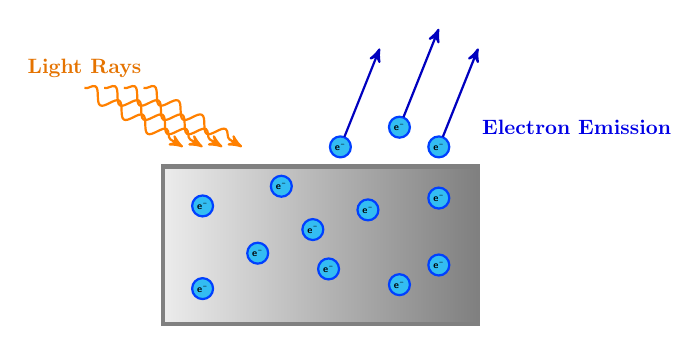
\begin{tikzpicture}[>=stealth',shorten >=0pt,auto,node distance=3cm,main node/.style={circle,thick, fill = white, scale=0.55, draw, font=\sffamily\large\bfseries}, photon/.style={decorate,decoration={snake,post length=1mm}}]
				%-------------------------start grid code ---------------------
					%\def\figWd{8.5};
					%\def\figHt{8.5};
					
					%\draw[step=0.5,very thin, black!15] (-0.5,-0.5) grid (\figWd,\figHt);
					
					%\draw[thick,->] (0,0) -- (\figWd,0) node[anchor=north west] {$x$};
					%\draw[thick,->] (0,0) -- (0,\figHt) node[anchor=south east] {$y$};
					
					%\foreach \x in {0,...,\figWd} 
					%\draw (\x cm,1pt) -- (\x cm,-1pt) node[anchor=north] {$\x$};
					%\foreach \y in {0,...,\figHt}
					%\draw (1pt,\y cm) -- (-1pt,\y cm) node[anchor=east] {$\y$};
				%--------------------------end grid code ----------------------
				%--------------------start metal bar code ---------------------
					\filldraw[draw=gray, ultra thick, left color = white!85!gray, right color = gray] (2,2) rectangle (6,4);
					
					\coordinate (e1) at (2.5,3.5);
					\node[blue,scale=0.3] (e1) at (e1) {\textcolor{black}{\textbf{\ce{e^-}}}};
					
					\coordinate (e2) at (3.5,3.75);
					\node[blue,scale=0.3] (e2) at (e2) {\textcolor{black}{\textbf{\ce{e^-}}}};
					
					\coordinate (e3) at (4.6,3.45);
					\node[blue,scale=0.3] (e3) at (e3) {\textcolor{black}{\textbf{\ce{e^-}}}};
					
					\coordinate (e4) at (5.5,3.6);
					\node[blue,scale=0.3] (e4) at (e4) {\textcolor{black}{\textbf{\ce{e^-}}}};
					
					\coordinate (e5) at (3.2,2.9);
					\node[blue,scale=0.3] (e5) at (e5) {\textcolor{black}{\textbf{\ce{e^-}}}};
					
					\coordinate (e6) at (4.1,2.7);
					\node[blue,scale=0.3] (e6) at (e6) {\textcolor{black}{\textbf{\ce{e^-}}}};
					
					\coordinate (e7) at (3.9,3.2);
					\node[blue,scale=0.3] (e7) at (e7) {\textcolor{black}{\textbf{\ce{e^-}}}};
					
					\coordinate (e8) at (5,2.5);
					\node[blue,scale=0.3] (e8) at (e8) {\textcolor{black}{\textbf{\ce{e^-}}}};
					
					\coordinate (e9) at (2.5,2.45);
					\node[blue,scale=0.3] (e9) at (e9) {\textcolor{black}{\textbf{\ce{e^-}}}};
					
					\coordinate (e10) at (5.5,2.75);
					\node[blue,scale=0.3] (e10) at (e10) {\textcolor{black}{\textbf{\ce{e^-}}}};
				%---------------------end metal bar code-----------------------
				%--------------------start light rays code ---------------------
					\coordinate (label1) at (1,5.25);
					\node[vertex,scale=0.75] (label1) at (label1) {\textcolor{orange!90!black}{\textbf{Light Rays}}};
										
					\foreach \x in {0,0.25,...,0.75}
						{\coordinate (x1) at (1 + \x, 5);
							\coordinate (x2) at (2.25 + \x, 4.25);
							\draw[->,photon,color=orange,thick] (x1) -- node[above left] {} (x2);
						};				
				%---------------------end light rays code -----------------------
				%--------------------start emitted electrons code ---------------------	
					\coordinate(E1_start) at (4.25, 4.25);
					\coordinate(E1_end) at (4.75, 5.5);					
					\node[blue,scale=0.3] (E1_start) at (E1_start) {\textcolor{black}{\textbf{\ce{e^-}}}};
					\path[->][black!25!blue,thick] (E1_start) edge [bend left=0] node{} (E1_end);
					
					\coordinate(E2_start) at (5, 4.5);
					\coordinate(E2_end) at (5.5, 5.75);					
					\node[blue,scale=0.3] (E2_start) at (E2_start) {\textcolor{black}{\textbf{\ce{e^-}}}};
					\path[->][black!25!blue,thick] (E2_start) edge [bend left=0] node{} (E2_end);
					
					\coordinate(E3_start) at (5.5, 4.25);
					\coordinate(E3_end) at (6, 5.5);					
					\node[blue,scale=0.3] (E3_start) at (E3_start) {\textcolor{black}{\textbf{\ce{e^-}}}};
					\path[->][black!25!blue,thick] (E3_start) edge [bend left=0] node{} (E3_end);
					
					\coordinate (label2) at (7.25,4.5);
					\node[vertex,scale=0.75] (label2) at (label2) {\textcolor{blue!90!black}{\textbf{Electron Emission}}};
				%---------------------end emitted electrons code ----------------------
			\end{tikzpicture}
		\end{center}
	\end{figure}
	
	\subsection*{Classical Prediction}	
		\begin{itemize}
			\item Low intensity (i.e., small amplitude) light will eject electrons at slower speeds (reasoned that light waves hit less "forcefully" when emitted at lower intensities)
			\item High intensity (i.e., large amplitude) light will eject electrons at higher speeds (reasoned that light waves hit more "forcefully" when emitted at higher intensities)
		\end{itemize}
	\subsection*{Actual Results}		
		\begin{itemize}
			\item The number of electrons emitted are proportional to the light intensity, but their kinetic energy (i.e., their speed) is independent of light intensity 
			\item The frequency $\nu$ associated with the emitted light waves must exceed a threshold $\nu_0$, even for high intensities 
			\item Furthermore, the KE associated with the emitted electrons depends on the $\nu$ 
			\item Scientist couldn't explain these results using classical mechanics and were puzzled by this and other paradoxes (eventually lead to the development of quantum mechanics)
		\end{itemize}
	\section*{Einstein's Prediction}
		\begin{itemize}
			\item In 1905, Einstein proposed that the energy associated with a light wave is proportional to the frequency of the light wave 
			\item He knew that by conservation of energy, that the energy of the light wave $E_p$ must be equal to the sum of the binding energy $\phi$ of the metal and the kinetic energy of the emitted electron $E_e$ 
				\begin{itemize}
					\item Let $\beta$ be an arbitrary proportionality constant (Note: this will end up being Planck's constant)
					\item Then, we can use the above assumptions to write $E_p = \beta \nu = \phi + E_e$
					\item Rewriting our equation gives $\boxed{E_e = \beta \nu - \phi}$
				\end{itemize}
		\end{itemize}			
\end{document}
